%-----------------------------------------------------------------------------%
\chapter{\babDua}
%-----------------------------------------------------------------------------%

%-----------------------------------------------------------------------------%
\section{\cc}
%-----------------------------------------------------------------------------%
\hspace{0.5cm} \cc, menurut definisi National Institute of Standards and Technology (NIST), merupakan suatu model komputasi yang menyediakan akses dan konfigurasi sumber daya komputasi seperti jaringan, server, penyimpanan, aplikasi, dan layanan secara on-demand, memungkinkan pelepasan yang cepat tanpa interaksi yang kompleks dengan penyedia layanan\cite{mell2009nist}. \cc\ bukanlah suatu teknologi spesifik, melainkan sebuah model yang menggambarkan operasional dan ekonomi untuk penyediaan serta penggunaan infrastruktur IT dan layanan terkait. Beberapa definisi cloud memiliki karakteristik umum yang sama, seperti \f{pay-per-use} (pembayaran sesuai dengan penggunaan), kapasitas yang elastis, layanan mandiri, dan abstraksi atau virtualisasi sumber daya\cite{Buyya_Broberg_Goscinski_2011}. NIST membagi model layanan cloud menjadi\cite{mell2009nist}:
\begin{enumerate}
    \item Software As A Service (SaaS)

    Konsumen dapat memanfaatkan kemampuan dengan menggunakan aplikasi penyedia yang beroperasi di dalam infrastruktur cloud. Aplikasi tersebut dapat diakses dari berbagai perangkat klien melalui antarmuka klien yang ringan, seperti browser web (contohnya, email berbasis web), atau antarmuka program. Pengguna tidak perlu mengelola atau mengontrol infrastruktur cloud yang mendasarinya, termasuk jaringan, server, sistem operasi, penyimpanan, atau bahkan kemampuan aplikasi individual, kecuali mungkin pada pengaturan konfigurasi aplikasi khusus pengguna yang terbatas.

    
    \item Platform As A Service (PaaS)

    Konsumen diberikan kemampuan untuk mendeploy aplikasi yang mereka buat atau peroleh ke infrastruktur cloud, menggunakan bahasa pemrograman, \f{library}, layanan, dan alat yang didukung oleh penyedia. Pengguna tidak perlu mengelola atau mengontrol infrastruktur cloud yang mendasarinya, termasuk jaringan, server, sistem operasi, atau penyimpanan. Meskipun begitu, pengguna tetap memiliki kendali atas aplikasi yang diimplementasikan dan mungkin dapat mengatur konfigurasi lingkungan hosting aplikasi.

    
    \item Infrastructure As A Service (IaaS)

    Kemampuan yang diberikan kepada konsumen adalah untuk menyediakan sumber daya pemrosesan, penyimpanan, jaringan, dan sumber daya komputasi dasar lainnya di mana konsumen dapat mendeploy dan menjalankan perangkat lunak sembarang, yang dapat mencakup sistem operasi dan aplikasi. Konsumen tidak mengelola atau mengendalikan infrastruktur awan yang mendasari tetapi memiliki kendali atas sistem operasi, penyimpanan, dan aplikasi yang didistribusikan; dan mungkin kendali terbatas terhadap beberapa komponen jaringan tertentu (misalnya, firewall host).
\end{enumerate}


%-----------------------------------------------------------------------------%
\section{Apache CloudStack}
%-----------------------------------------------------------------------------%
\begin{figure}
	\centering
	
\includegraphics[width=0.70\textwidth]
		{assets/pics/apache_cloudstack_with_cloud_monkey.jpg}
	\caption{Logo Apache CloudStack}
	\label{fig:LogoApacheCloudStack}
\end{figure}
\hspace{0.5cm} Apache CloudStack adalah perangkat lunak \oss\ yang dirancang untuk mendeploy dan mengelola jaringan besar mesin virtual, sebagai platform komputasi awan berbasis Infrastructure as a Service (IaaS) yang sangat tersedia dan dapat \f{scaleable}\cite{cloudstackabout}. Pada Gambar \ref{fig:LogoApacheCloudStack} adalah logo dari Apache Cloudstack. CloudStack digunakan oleh sejumlah penyedia layanan untuk menawarkan layanan cloud publik, dan oleh banyak perusahaan untuk menyediakan penawaran cloud \f{on-premise} (pribadi), atau sebagai bagian dari solusi cloud hybrid\cite{cloudstackabout}.

CloudStack adalah solusi siap pakai yang mencakup seluruh "stack" fitur yang paling diinginkan oleh organisasi dengan IaaS cloud: orkestrasi komputasi, Jaringan sebagai Layanan, manajemen pengguna dan akun, dan antarmuka Pengguna (UI) yang baik\cite{cloudstackabout}.

CloudStack saat ini mendukung hypervisor paling populer: VMware, KVM, Citrix XenServer, Xen Cloud Platform (XCP), Oracle VM server, dan Microsoft Hyper-V\cite{cloudstackabout}.

Pengguna dapat mengelola cloud mereka dengan antarmuka web yang mudah digunakan, alat \f{commandline}, dan/atau API RESTful yang lengkap. Selain itu, CloudStack menyediakan API yang kompatibel dengan AWS EC2 dan S3 untuk organisasi yang ingin mendeploy cloud secara hybrid\cite{cloudstackabout}.

CloudStack, yang awalnya dikembangkan oleh Cloud.com, diakuisisi oleh Citrix pada tahun 2011 dan diserahkan kepada Apache Software Foundation pada tahun 2012. Pengembangan saat ini diatur oleh Apache Foundation dengan kode yang tersedia di bawah lisensi Apache 2.0\cite{techtargetcloudstack}.


%-----------------------------------------------------------------------------%
\section{Hypervisor}
%-----------------------------------------------------------------------------%
\hspace{0.5cm} Sebuah hypervisor adalah perangkat lunak atau perangkat keras yang digunakan untuk menciptakan dan mengelola mesin virtual. Juga dikenal sebagai \f{'Virtual Machine Monitor'} atau VMM, hypervisor memungkinkan satu server fisik menjalankan beberapa mesin virtual, mengatasi keterbatasan satu sistem operasi pada satu server. Hypervisor dapat berupa perangkat keras atau program, dan fungsinya adalah menciptakan, memonitor, dan mengelola mesin-mesin virtual\cite{MacPherson_2023}.

\begin{figure}
	\centering
	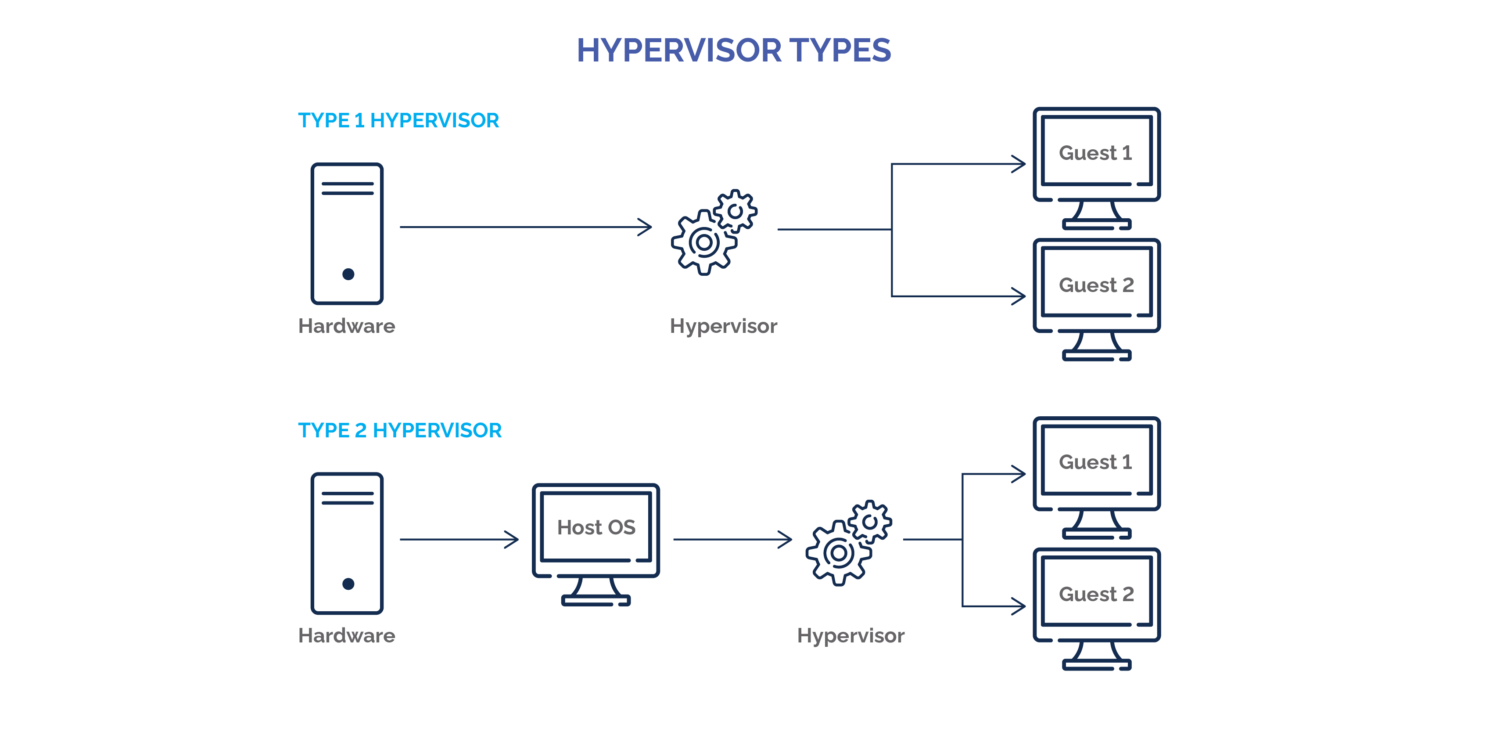
\includegraphics[width=1\textwidth]
		{assets/pics/type-1-hypervisor-vs-type-2.png}
	\caption{Hypervisor Type 1 vs Type 2}
	\label{fig:HypervisorType1vsType2}
\end{figure}

Pada Gambar \ref{fig:HypervisorType1vsType2} diperlihatkan diagram sederhana perbedaan daripada Hypervisor tipe 1 dan Hypervisor tipe 2. Hypervisor tipe 1 dan tipe 2 merupakan perangkat lunak yang digunakan untuk menjalankan satu atau lebih \vm\ (VM) pada satu mesin fisik. \vm\ adalah replika digital dari mesin fisik, menciptakan lingkungan komputasi terisolasi yang pengguna alami sebagai sepenuhnya independen dari perangkat keras yang mendasarinya\cite{hypervisor1vs2}. Hypervisor mengelola dan mengalokasikan sumber daya fisik ke VM dan berkomunikasi dengan perangkat keras di latar belakang. Hypervisor tipe 1 ditempatkan di atas server tanpa sistem operasi dan memiliki akses langsung ke sumber daya perangkat keras, sehingga dikenal juga sebagai \f{bare metal} hypervisor. Sebaliknya, hypervisor tipe 2 adalah aplikasi yang diinstal pada sistem operasi host dan juga dikenal sebagai \f{hosted} atau \f{embedded} hypervisor\cite{hypervisor1vs2}. 


%-----------------------------------------------------------------------------%
\section{KVM \f{(Kernel-Based Virtual Machine)}}
%-----------------------------------------------------------------------------%

\hspace{0.5cm} KVM (Kernel-based Virtual Machine) merupakan modul virtualisasi \oss\ dan gratis dalam kernel Linux yang memungkinkan kernel berfungsi sebagai hypervisor. KVM adalah hypervisor tipe 1 atau biasa juga disebut sebagai hypervisor \f{bare metal}. KVM memungkinkan mesin host menjalankan beberapa lingkungan virtual terisolasi yang disebut sebagai guest atau \vm\ (VM).KVM (Kernel-based Virtual Machine) merupakan modul virtualisasi sumber terbuka dan gratis dalam kernel Linux yang memungkinkan kernel berfungsi sebagai hypervisor. Ini adalah tipe-1 (bare-metal) hypervisor yang memungkinkan mesin host menjalankan beberapa lingkungan virtual terisolasi yang disebut sebagai guest atau mesin virtual (VM).

KVM telah disatukan ke dalam kernel Linux utama pada versi 2.6.20, yang dirilis pada 5 Februari 2007. Untuk dapat berjalan, KVM memerlukan prosesor dengan ekstensi virtualisasi perangkat keras, seperti Intel VT atau AMD-V. KVM menyediakan abstraksi perangkat tetapi tidak ada emulasi prosesor. Modul ini mengekspos antarmuka /dev/kvm, yang dapat digunakan oleh mode pengguna untuk menyiapkan ruang alamat VM guest.

KVM mendukung virtualisasi perangkat keras untuk berbagai sistem operasi guest, termasuk BSD, Solaris, Windows, Haiku, ReactOS, Plan 9, dan lainnya. Sebagai bagian dari kernel Linux, KVM langsung mengambil manfaat dari setiap fitur baru, perbaikan, dan kemajuan Linux tanpa perlu rekayasa tambahan.

Dalam pengaturan KVM, CPU virtual dari VM diimplementasikan sebagai thread (disebut "virtual CPU" atau vcpu) yang dijadwalkan oleh \f{Linux Kernel Scheduler}. KVM pada dasarnya adalah pengemudi untuk ekstensi virtualisasi processor. Setiap kali \f{Linux Scheduler} memilih tugas untuk dijalankan pada CPU fisik, dan tugas tersebut dikerjakan oleh CPU virtual dari VM, KVM "dihubungi" untuk memastikan bahwa yang sebenarnya berjalan di perangkat keras adalah program dari OS guest\cite{Abeni2020}.

\begin{figure}
	\centering
	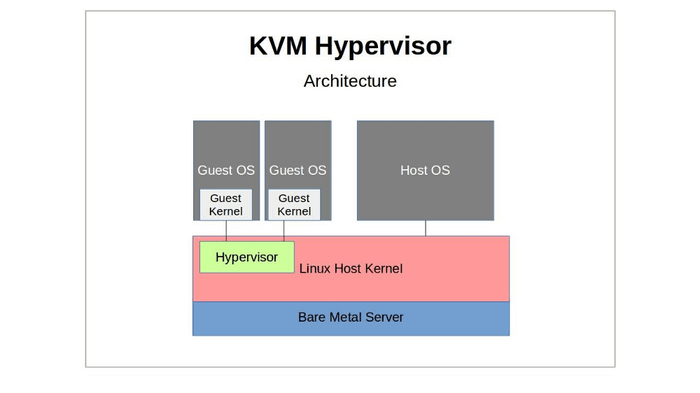
\includegraphics[width=1\textwidth]
		{assets/pics/xen-kvm.png}
	\caption{Hypervisor Type 1 vs Type 2}
	\label{fig:xen-kvm}
\end{figure}

Pada Gambar \ref{fig:xen-kvm} adalah struktur daripada hypervisor KVM. KVM berjalan langsung pada kernel linux host dan membagikan resourcenya kepada guest \vm, sedangkan sistem operasi host berjalan langsung diatas kernel host. Sistem operasi host dapat melakukan konfigurasi kepada \vm\ yang menggunakan hypervisor miliknya.

%-----------------------------------------------------------------------------%
\section{\f{Virtual Machine}}
%-----------------------------------------------------------------------------%

\hspace{0.5cm} Virtual Machine (VM) adalah sebuah lingkungan komputasi yang dibuat secara virtual di dalam sebuah komputer fisik (host)\cite{Pradilla2016}. VM ini berfungsi seperti sebuah komputer independen yang dapat menjalankan sistem operasi dan aplikasi seperti komputer fisik biasa, tetapi semuanya berjalan dalam lingkungan virtual yang terisolasi di dalam host fisik. Setiap \vm (VM) menjalankan sistem operasi secara independen dan beroperasi terpisah dari VM lainnya, bahkan ketika semuanya berjalan pada host yang sama. Perangkat lunak yang dikenal sebagai hypervisor atau \vmm (VMM) memungkinkan kita untuk menjalankan berbagai sistem operasi yang berbeda secara bersamaan pada \vm yang berbeda. VM memiliki beberapa keunggulan dibandingkan dengan mesin fisik, termasuk kemampuan untuk menjalankan beberapa lingkungan sistem operasi pada satu komputer fisik, mendukung aplikasi \f{legacy}, dan menyediakan opsi pemulihan dalam situasi bencana. VM digunakan untuk berbagai keperluan, seperti \cc, pengujian sistem operasi baru, dan menjalankan beberapa aplikasi pada satu mesin fisik\cite{ibmWhatVirtualMachine}.

\begin{figure}
	\centering
	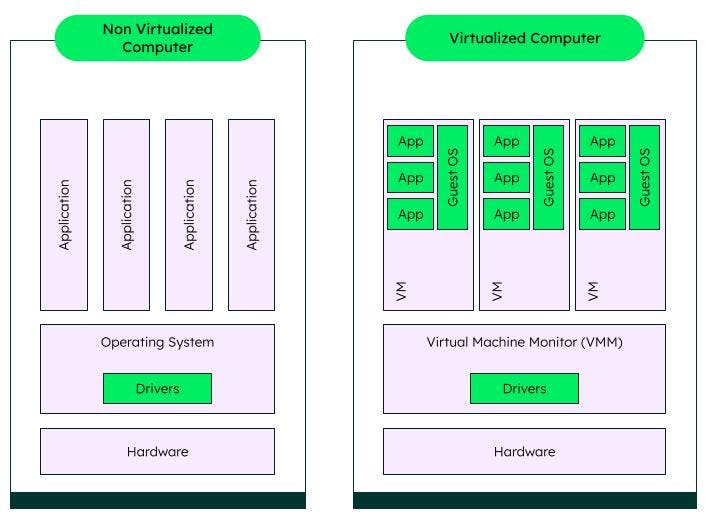
\includegraphics[width=1\textwidth]
	{assets/pics/vm-diagram.jpg}
	\caption{Perbedaan Komputasi Tanpa Virtualisasi dengan Virtualisasi}
	\label{fig:vm-diagram}
\end{figure}

Terdapat perbedaan dalam cara berjalan antara komputer tanpa virtualisasi (host) dan komputer yang divirtualisasi (guest) atau \vm. Pada Gambar 2.4, dapat diperlihatkan bahwa pada komputer tanpa virtualisasi, sistem operasinya berjalan langsung di atas perangkat keras, dengan driver yang berfungsi sebagai jembatan, sehingga aplikasi dapat berjalan langsung di atas sistem operasi tersebut. Di sisi lain, pada komputer yang divirtualisasi, sistem operasinya berjalan di atas VMM atau Virtual Machine Monitor, di mana satu VMM dapat menjalankan banyak sistem operasi guest.

%-----------------------------------------------------------------------------%
\section{virsh}
%-----------------------------------------------------------------------------%

\hspace{0.5cm} virsh adalah \f{command line tool} yang merupakan bagian dari \f{library} libvirt dan secara utama digunakan untuk mengelola dan berinteraksi dengan teknologi virtualisasi pada sistem Linux, khususnya KVM (Kernel-based Virtual Machine) dan QEMU (Quick Emulator), dan mendukung hypervisor lainnya seperti Xen, LXC, OpenVZ, VirtualBox, dan VMware ESX\cite{libvirtLibvirtVirsh}.

Secara sederhana penggunaan virsh adalah seperti ini
\begin{center}
	\begin{verbatim}
		virsh [OPTION]... <command> <domain> [ARG]...
	\end{verbatim}
\end{center}

%-----------------------------------------------------------------------------%
\section{\latex~Secara Singkat}
%-----------------------------------------------------------------------------%
Definisi dari LaTeX \citep{lankton2008introduction} adalah: \\ 
\begin{tabular}{| p{13cm} |}
	\hline 
	\\
	LaTeX is a family of programs designed to produce publication-quality 
	typeset documents. It is particularly strong when working with 
	mathematical symbols. \\	
	The history of LaTeX begins with a program called TEX. In 1978, a 
	computer scientist by the name of Donald Knuth grew frustrated with the 
	mistakes that his publishers made in typesetting his work. He decided 
	to create a typesetting program that everyone could easily use to 
	typeset documents, particularly those that include formulae, and made 
	it freely available. The result is TEX. \\	
	Knuth's product is an immensely powerful program, but one that does 
	focus very much on small details. A mathematician and computer 
	scientist by the name of Leslie Lamport wrote a variant of TEX called 
	LaTeX that focuses on document structure rather than such details. \\
	\\
	\hline
\end{tabular}

\vspace*{0.8cm}

Contoh sitasi lainnya menggunakan \verb|\citep| adalah saat kita mau mensitasi pekerjaan tentang \textit{machine learning} \citep{chin2000learning} dan \textit{dynamic programming} \citep{barto1995learning}. \\

Dokumen \latex~sangat mudah, seperti halnya membuat dokumen teks biasa. Ada 
beberapa perintah yang diawali dengan tanda '\bslash'. 
Seperti perintah \bslash\bslash~yang digunakan untuk memberi baris baru. 
Perintah tersebut juga sama dengan perintah \bslash newline. 
Pada bagian ini akan sedikit dijelaskan cara manipulasi teks dan 
perintah-perintah \latex~yang mungkin akan sering digunakan. 
Jika ingin belajar hal-hal dasar mengenai \latex, silahkan kunjungi: 

\begin{itemize}
	\item \url{http://frodo.elon.edu/tutorial/tutorial/}, atau
	\item \url{http://www.maths.tcd.ie/~dwilkins/LaTeXPrimer/}
\end{itemize}


%-----------------------------------------------------------------------------%
\section{\latex~Kompiler dan IDE}
%-----------------------------------------------------------------------------%
Agar dapat menggunakan \latex~(pada konteks hanya sebagai pengguna), Anda 
tidak perlu banyak tahu mengenai hal-hal didalamnya. 
Seperti halnya pembuatan dokumen secara visual (contohnya Open Office (OO) 
Writer), Anda dapat menggunakan \latex~dengan cara yang sama. 
Orang-orang yang menggunakan \latex~relatif lebih teliti dan terstruktur 
mengenai cara penulisan yang dia gunakan, \latex~memaksa Anda untuk seperti 
itu.  

Kembali pada bahasan utama, untuk mencoba \latex~Anda cukup mendownload 
kompiler dan IDE. Saya menyarankan menggunakan Texlive dan Texmaker. 
Texlive dapat didownload dari \url{http://www.tug.org/texlive/}. 
Sedangkan Texmaker dapat didownload dari 
\url{http://www.xm1math.net/texmaker/}. 
Untuk pertama kali, coba buka berkas thesis.tex dalam template yang Anda miliki 
pada Texmaker. 
Dokumen ini adalah dokumen utama. 
Tekan F6 (PDFLaTeX) dan Texmaker akan mengkompilasi berkas tersebut menjadi 
berkas PDF. 
Jika tidak bisa, pastikan Anda sudah menginstall Texlive. 
Buka berkas tersebut dengan menekan F7. 
Hasilnya adalah sebuah dokumen yang sama seperti dokumen yang Anda baca saat 
ini. 


%-----------------------------------------------------------------------------%
\section{Bold, Italic, dan Underline}
%-----------------------------------------------------------------------------%
Hal pertama yang mungkin ditanyakan adalah bagaimana membuat huruf tercetak 
tebal, miring, atau memiliki garis bawah. 
Pada Texmaker, Anda bisa melakukan hal ini seperti halnya saat mengubah dokumen 
dengan OO Writer. 
Namun jika tetap masih tertarik dengan cara lain, ini dia: 

\begin{itemize}
	\item \bo{Bold} \\
		Gunakan perintah \bslash textbf$\lbrace\rbrace$ atau 
		\bslash bo$\lbrace\rbrace$. 
	\item \f{Italic} \\
		Gunakan perintah \bslash textit$\lbrace\rbrace$ atau 
		\bslash f$\lbrace\rbrace$. 
	\item \underline{Underline} \\
		Gunakan perintah \bslash underline$\lbrace\rbrace$.
	\item $\overline{Overline}$ \\
		Gunakan perintah \bslash overline. 
	\item $^{superscript}$ \\
		Gunakan perintah \bslash $\lbrace\rbrace$. 
	\item $_{subscript}$ \\
		Gunakan perintah \bslash \_$\lbrace\rbrace$. 
\end{itemize}

Perintah \bslash f dan \bslash bo hanya dapat digunakan jika package 
uithesis digunakan. 


%-----------------------------------------------------------------------------%
\section{Memasukan Gambar}
%-----------------------------------------------------------------------------%
Setiap gambar dapat diberikan caption dan diberikan label. Label dapat 
digunakan untuk menunjuk gambar tertentu. 
Jika posisi gambar berubah, maka nomor gambar juga akan diubah secara 
otomatis. 
Begitu juga dengan seluruh referensi yang menunjuk pada gambar tersebut. 
Contoh sederhana adalah \pic~\ref{fig:testGambar}. 
Silahkan lihat code \latex~dengan nama bab2.tex untuk melihat kode lengkapnya. 
Harap diingat bahwa caption untuk gambar selalu terletak dibawah gambar. 

\begin{figure}
	\centering
	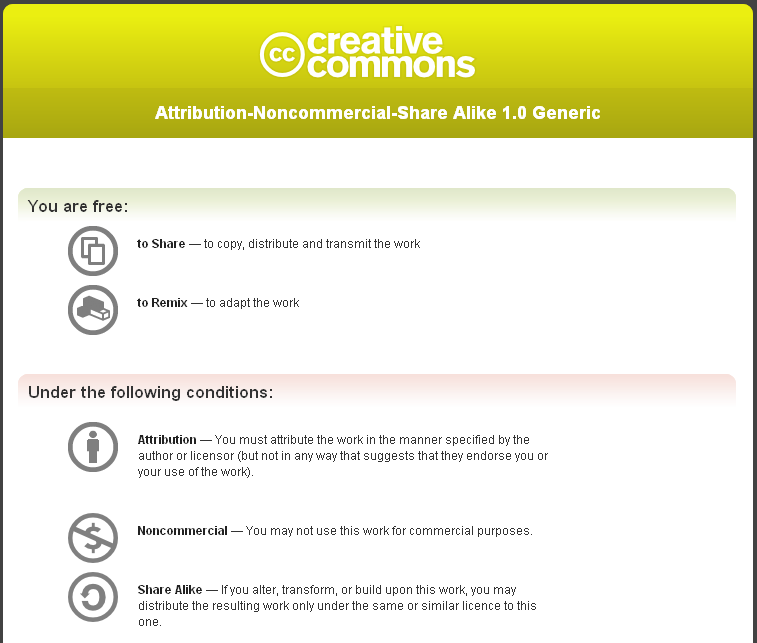
\includegraphics[width=0.50\textwidth]
		{assets/pics/creative_common.png}
	\caption{\license.}
	\label{fig:testGambar}
\end{figure}


%-----------------------------------------------------------------------------%
\section{Membuat Tabel}
%-----------------------------------------------------------------------------%
Seperti pada gambar, tabel juga dapat diberi label dan caption. 
Caption pada tabel terletak pada bagian atas tabel. 
Contoh tabel sederhana dapat dilihat pada \tab~\ref{tab:tab1}.

\begin{table}
	\centering
	\caption{Contoh Tabel}
	\label{tab:tab1}
	\begin{tabular}{| l | c r |}
		\hline
		& kol 1 & kol 2 \\ 
		\hline
		baris 1 & 1 & 2 \\
		baris 2 & 3 & 4 \\
		baris 3 & 5 & 6 \\
		jumlah  & 9 & 12 \\
		\hline
	\end{tabular}
\end{table}

Ada jenis tabel lain yang dapat dibuat dengan \latex~berikut 
beberapa diantaranya. 
Contoh-contoh ini bersumber dari 
\url{http://en.wikibooks.org/wiki/LaTeX/Tables}

\begin{table}
	\centering
	\caption{An Example of Rows Spanning Multiple Columns}
	\label{row.spanning}
	\begin{tabular}{|l|l|*{6}{c|}}
  		\hline % create horizontal line
  		No & Name & \multicolumn{3}{|c|}{Week 1} & \multicolumn{3}{|c|}{Week 2} \\
  		\cline{3-8} % create line from 3rd column till 8th column
  		& & A & B & C & A & B & C\\
  		\hline
  		1 & Lala & 1 & 2 & 3 & 4 & 5 & 6\\
  		2 & Lili & 1 & 2 & 3 & 4 & 5 & 6\\
  		3 & Lulu & 1 & 2 & 3 & 4 & 5 & 6\\
  		\hline
	\end{tabular}
\end{table}

\begin{table}
	\centering
	\caption{An Example of Columns Spanning Multiple Rows}
	\label{column.spanning}
	\begin{tabular}{|l|c|l|}
		\hline
		Percobaan & Iterasi & Waktu \\
		\hline
		Pertama & 1 & 0.1 sec \\ \hline
		\multirow{2}{*}{Kedua} & 1 & 0.1 sec \\
 		& 3 & 0.15 sec \\ 
 		\hline
		\multirow{3}{*}{Ketiga} & 1 & 0.09 sec \\
 		& 2 & 0.16 sec \\
 		& 3 & 0.21 sec \\ 
 		\hline
	\end{tabular}
\end{table}

\begin{table}
	\centering
	\caption{An Example of Spanning in Both Directions Simultaneously}
	\label{mix.spanning}
	\begin{tabular}{cc|c|c|c|c|}
		\cline{3-6}
		& & \multicolumn{4}{|c|}{Title} \\ \cline{3-6}
		& & A & B & C & D \\ \hline
		\multicolumn{1}{|c|}{\multirow{2}{*}{Type}} &
		\multicolumn{1}{|c|}{X} & 1 & 2 & 3 & 4\\ \cline{2-6}
		\multicolumn{1}{|c|}{}                        &
		\multicolumn{1}{|c|}{Y} & 0.5 & 1.0 & 1.5 & 2.0\\ \cline{1-6}
		\multicolumn{1}{|c|}{\multirow{2}{*}{Resource}} &
		\multicolumn{1}{|c|}{I} & 10 & 20 & 30 & 40\\ \cline{2-6}
		\multicolumn{1}{|c|}{}                        &
		\multicolumn{1}{|c|}{J} & 5 & 10 & 15 & 20\\ \cline{1-6}
	\end{tabular}
\end{table}

